\documentclass[10pt, a4paper]{article}
\usepackage{multicol}
\usepackage{listings}
\usepackage{geometry}
\usepackage{graphicx}
\usepackage{caption}

\graphicspath{{img}}

\pagenumbering{gobble}
\date{}

\begin{document}

NAMA: Radinal Shidiq Saragih

KELAS: IF C 2023

NPM: 5520123104

\begin{enumerate}
  \item Pallete

    \begin{multicols}{2}
      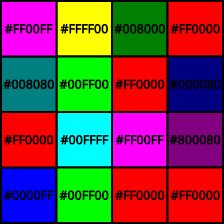
\includegraphics[scale=0.8]{PALLETE.png}

    \begin{center}

      \begin{itemize}
        \item Resolusi: 4 x 4
        \item Bit depth: 24bit
      \end{itemize}

        Ukuran File = width x height x Bit Depth

        Ukuran File = 4 x 4 x 24 = 384 Bit 

        Ukuran File = (384 / 8) = 48 Byte

    \end{center}

    \end{multicols}

  \item Pallete Berindeks

    \begin{multicols}{2}
      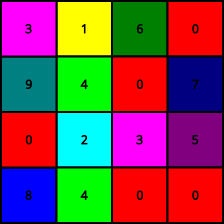
\includegraphics[scale=0.8]{PALLETE2.png}
      \begin{center}
        \begin{tabular} {| c | c |}
          \hline
          INDEX & WARNA \\
          \hline
            0 & \#FF0000 (255, 0, 0)   \\
          \hline
            1 & \#FFFF00 (255, 255, 0) \\
          \hline
            2 & \#00FFFF (0, 255, 255) \\
          \hline
            3 & \#FF00FF (255, 0, 255) \\
          \hline
            4 & \#00FF00 (0, 255, 0)   \\
          \hline
            5 & \#800080 (128, 0, 128) \\
          \hline
            6 & \#008000 (0, 128, 0)   \\
          \hline
            7 & \#000080 (0, 0, 128)   \\
          \hline
            8 & \#0000FF (0, 0, 255)   \\
          \hline
            9 & \#008080 (0, 128, 128) \\
          \hline
        \end{tabular}
      \end{center}
    \end{multicols}

    \begin{center}

      \begin{itemize}
        \item Resolusi: 4 x 4
        \item Bit depth: 24bit
        \item Jumlah Warna: 9

        \item Ukuran Byte Per-Pixel = Bit Depth / 8 (1 Byte = 8 bit)

              Ukuran Byte Per-Pixel = 24 / 8 = 3 Byte
      \end{itemize}

        \vspace{0.2cm}

        Ukuran File = width x height x Bit Depth

        Ukuran File = 4 x 4 x 24 = 384 Bit 

        Ukuran File = (384 / 8) = 48 Byte

        \vspace{0.2cm}

        Ukuran Pallete = Jumlah Warna x Ukuran Pixel per Byte

        Ukuran Pallete = 9 x 3 = 27 Byte

        \vspace{0.2cm}

        Total Ukuran Gambar = Ukuran File + Ukuran Pallete

        Total Ukuran Gambar = 48 + 27 = 75 Byte


    \end{center}


\end{enumerate}

\end{document}
